\documentclass[a4paper]{article}

\usepackage[english]{babel}
\usepackage[utf8x]{inputenc}
\usepackage[T1]{fontenc}

\usepackage[a4paper,top=3cm,bottom=2cm,left=3cm,right=3cm,marginparwidth=1.75cm]{geometry}

\usepackage{amsmath}
\usepackage{graphicx}
\usepackage[colorinlistoftodos]{todonotes}
\usepackage[colorlinks=true, allcolors=blue]{hyperref}
\usepackage{capt-of}
\usepackage{floatrow}
\floatsetup{heightadjust=object}
\newfloatcommand{capbtabbox}{table}[][\FBwidth]

\newcommand{\note}[1]{\marginpar{#1}}

%\setlength{\parindent}{0pt}

\title{Decision Trees\\\large{Mathematical Aspects of Machine Learning}}
\author{Florian Hartmann, Yu He}
\date{July 17, 2017}

\begin{document}
\maketitle

\section{Introduction}

Decision trees are a popular method in supervised Machine Learning. For this project phase, we decided to explore them in more detail and to apply them to some interesting datasets. Primarily, our motivation behind this was that decision trees are very interpretable. Part of the project is analyzing datasets, and we concluded that choosing an interpretable method would be quite helpful for doing that.

Before diving into the dataset analysis, this section introduces the foundational ideas behind decision trees. Section 2 quickly deals with our decision tree visualizations. After having understood how to use decision trees, the more important question of how to build them is discussed in the next section, by looking at two popular algorithms. Section 4 deals with a popular heuristic for choosing the features that are used to make decisions.
The section afterwards explains how ensemble methods can be used to combat overfitting. Finally, two datasets are analyzed using decision trees.

A toy decision tree using weather features can be found in Figure \ref{fig:simple}. Decision trees consist of two types of nodes: First of all, internal nodes (i.e.\ nodes that are not leafs) make decisions based on features. Depending on the outcome of the decision, a different child node is visited next. At the bottom of the tree, there are leafs: They make very simple predictions, e.g.\ by just constantly predicting the same answer, or by using a linear classifier. In the visualization, internal nodes are displayed using ellipses, leafs using rectangles. To make a prediction, a path down the decision tree is traversed until a leaf is reached. The leaf node is then asked to make the final prediction.

In the example in Figure~\ref{fig:simple}, different weather conditions are evaluated in the internal nodes, until, finally, a decision is made in the leaf on whether to go outside or stay inside.

\begin{figure}[h]
	\centering
	\includegraphics[scale=0.4]{introduction.jpg}
    \caption{A simple decision tree}
    \label{fig:simple}
\end{figure}

Another way to think about this is that decision trees repeatedly split the input space, until the individual partitions allow for simple predictions. In computer science, this is known as a divide and conquer strategy. By making several subsequent decisions based on each other, nonlinear decision boundaries can easily be created.

There are many other useful traits of decision trees. For example, users have to perform very little data preprocessing. Feature values do not need to be normalized at all, and some decision tree algorithms can even deal with missing values by themselves. Decision trees can also handle multi-class datasets without any changes.

As mentioned earlier, decision trees allow for easy interpretation. In contrast to other Machine Learning methods like neural networks, it is very clear why a prediction was made. For many applications, for example in the medical world, this interpretability is very important and a great advantage of decision trees.

By now it should be obvious that decision trees describe their training data very clearly. However, this also leads to the great disadvantage that decision trees overfit easily. In many cases, they learn to describe the training data exactly, and their predictions do not generalize well to unseen data. Several sections of this report deal with methods that aim to reduce this problem.

Finally, it is worth noting that we focus on classification in this report. Nevertheless, decision trees can also be used for regression, e.g.\ by using linear regression models in the leafs.

\section{Drawing Decision Trees}

Before diving into building decision trees, we quickly want to mention that we also wrote code for visualizing decision trees. This allows us to see whether our algorithm actually produces something reasonable. Furthermore, we can use the visualizations to analyze our datasets. All visualizations in this report were generated by our code.

Technically, drawing the tree is based on the \emph{pydot} graphics library. To traverse all nodes of the tree, a breadth-first search is performed, and information about all the nodes is collected.

\begin{figure}[h]
	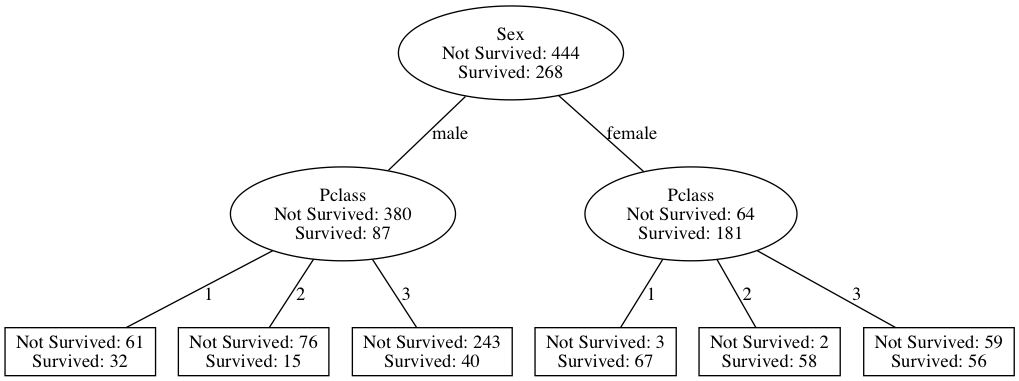
\includegraphics[scale=0.3]{titanic-depth2-id3.png}
    \caption{Titanic decision tree (ID3)}
    \label{fig:drawing-titanic}
\end{figure}

An example of how the result might look like is given in Figure~\ref{fig:drawing-titanic}. Internal nodes are drawn using ellipses, leafs using rectangles. The first line of an internal node tells us what feature the split is based on, the edge descriptions correspond to the possible feature values. All further lines in internal nodes and leafs describe the label distributions (in this decision tree, whether a passenger survived or not).

\section{Constructing Decision Trees}

\subsection{ID3}

ID3 (Iterative Dichotomiser 3) \cite{mitchell1997machine, quinlan1986induction} is a straight-forward approach to building decision trees. We decided to start with this algorithm because it allows for a gentle introduction to the fundamental ideas behind building decision trees.
The fact that it is quite simple also means that it has some serious drawbacks, and generally should not be used in production. We will explain these shortcomings and address the most important ones in later sections of the report.

Generally, ID3 uses the ideas introduced in the previous section.
As described there, we distinguish between two types of nodes. Internal nodes make the decision which child node to visit next, and leafs perform constant predictions.
To build a decision tree using ID3, a recursive strategy is followed: The training data is repeatedly split until a new node gets training data that is suitable for making a constant prediction.

In the following, both types of nodes are discussed in more detail, starting with internal nodes.

\subsubsection{Internal nodes: Making decisions}

In ID3, the input data is always split based on a single feature. For each possible value of that feature a new child node is created.
In other words, if a split is made on a feature that allows $k$ different values, then the node will have exactly $k$ child nodes.
The child nodes then build their own subtrees using the subset of training data from the parent node that has the respective value in the selected feature.

Here the first serious drawback of ID3 becomes apparent: Splitting on all possible values only works well for features with a handful of different values. For a continuous variable like \emph{age} this approach would work terribly. In our opinion, this is also the major shortcoming of ID3. In Section \ref{subsec:c45}, we will see an algorithm that deals with continuous features in a smarter way.

\subsubsection{Leafs: Stopping the recursion}

At some point, the recursion has to end, which means a node does not grow its own subtree but is turned into a leaf. The leaf then constantly predicts the same answer. Which answer to predict is based on the training data it received.

There are various reasons why a node might be turned into a leaf. The simplest one is that all data points it received have the same label. In this case, there is no reason to split the data further, and the node can be turned into a leaf which predicts this label. A similar case is that the training data does not allow for any further splits, e.g.\ because all data points are equal to each other but have different labels. In this case, the most common label is predicted.

Another case is that there is just no training data available. We always create a new node for each possible value of a feature. If we are deep in the tree and split on a feature that can have many different values, there might be no more training data for some values. If this happens, the most common label of the parent node is predicted.

There are other cases where we might want to stop the recursion. We will come back to these in Section \ref{subsec:id3-depth}.

\subsubsection{Selecting the feature to split on}

Of course, now the major remaining question is how find the best feature to split on. ID3 follows a greedy strategy for this. For each feature, it evaluates how well the classes would be divided in the next step if a split based on this feature would be performed. Then, the feature where this worked best is chosen. Of course, this greedy strategy could mean that a very good combination of subsequent splits is missed, because we were too greedy in the beginning.

To find the feature which produces the best division in the next step, different heuristics can be used. The easiest one is misclassification: We just assume that the next node will predict the most common label, and calculate how accurate it would be by doing this. Then, the feature with the lowest misclassification rate is chosen.

A more popular heuristic, that is also used in ID3, is entropy with information gain. In a nutshell, entropy measures uncertainty, i.e.\ it wants nodes to receive data points that mostly have the same label so that a prediction can be made with a lot of certainty. Because entropy and information gain are not only used in ID3, but also in C4.5, a more thorough description of them is given in Section~\ref{sec:entropy}.

Another important idea to mention is that in ID3, each feature should only be used once for splitting. Because we split based on all possible values, the data of each child only has one distinct value for each feature that was already split on. Hence, it does not make sense to split on these features again.

\subsubsection{Limiting the tree depth}
\label{subsec:id3-depth}

Overfitting is a huge problem when using decision trees. It can happen very easily that the training data is described perfectly. However, this description might contain so much random noise that predictions do not generalize well to previously unseen data points.

In most Machine Learning algorithms, a very common way to combat overfitting is regularization: By adding additional constraints, the model is forced to be simpler. A simpler model means there is less capacity for remembering information from the training data, which has the effect that only the most important information is represented in the model.

For decision trees, the primary way of adding regularization is to limit the depth of the tree. Because we split on each feature exactly once, limiting the tree depth in ID3 is equivalent to limiting the maximum number of features that should be used for one prediction. If only a small tree depth is allowed, it means that only the most important features are considered. When the maximum depth is reached, leafs are created that predict the most common label of the data they got.

Of course, the optimal tree depth highly depends on the dataset being used. Because of this, tree depth is a hyperparameter that needs be optimized using a method like grid search.

Another way to limit the tree depth is to only perform a split if it helps to divide the classes much better. The intuition behind this is that other splits tend to introduce more model complexity without directly improving the predictive power of the model.

However, these other splits are sometimes necessary to get a good division in the next split afterwards. One extreme example for this, which we found when testing our implementation, is the $\mathit{xor}$ dataset, see Table \ref{fig:xor-table}. We have two features, $a$ and $b$, that take the values of $0$ and $1$. The label is computed using the $\mathit{xor}$ function. Ideally, our decision tree should look like the one in Figure \ref{fig:xor-tree}.

By looking at this decision tree, it becomes apparent that the first split does not directly help to separate the classes. The root node had an equal number of data points from both classes, as do its children. By only looking at these three nodes, one might think that the split should not have been performed. However, by doing this split we can perfectly divide the classes in the next step, reaching an accuracy of 100\%, instead of just 50\%. To conclude, because of the greedy strategy, we cannot directly know whether a split should be performed or not.

\begin{figure}
\begin{floatrow}
\ffigbox{%
  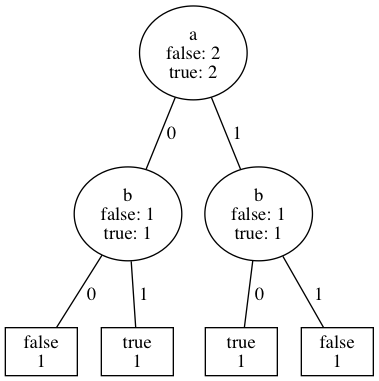
\includegraphics[scale=0.4]{xor.png}%
}{%
\caption{$\mathit{xor}$ decision tree}%
	\label{fig:xor-tree}
}
\capbtabbox{%
  \begin{tabular}{c|c|c}
      \textbf{a} & \textbf{b} &  \textbf{y = a xor b} \\
      \hline
      0 & 0 & false \\
      0 & 1 & true  \\
      1 & 0 & true \\
      1 & 1 & false
  \end{tabular}
}{%
\caption{$\mathit{xor}$ truth table}%
	\label{fig:xor-table}
}
\end{floatrow}
\end{figure}

\subsection{C4.5}
\label{subsec:c45}

C4.5~\cite{wu2008top, quinlan2014c4, mitchell1997machine} is a more advanced decision tree algorithm that was designed to fix many of ID3's shortcomings. It was created by Ross Quinlan, who also invented ID3. Quinlan wrote an entire book~\cite{quinlan2014c4} on C4.5, so to reimplement all ideas and variations of C4.5 is beyond the scope of this project. Instead, we will focus on the three ideas that we consider to be the most central ones.

\subsubsection{Continuous features}

As we saw in the previous section, ID3 can only deal well with discrete features. However, most datasets contain continuous features. Always throwing these features away, or manually converting them into discrete features, is of course not an acceptable solution. This is not necessary in C4.5, as it can directly deal with continuous features.

Before we start explaining how the splitting works, it is worth taking a moment to think about how the algorithm actually knows whether a feature is discrete or continuous. Because we are only working on a finite set of samples, it is impossible to always automatically detect this correctly. One could imagine checking how many different values a feature has, and then just considering it as continuous if it has more than a certain number of different values. However, this process is very error-prone. Zip codes would probably be considered continuous, although they come from a discrete set. In the end, we just decided that the user should tell the algorithm which features to treat as continuous features.

If a feature is continuous, we, of course, do not want to split on all possible values. Instead, C4.5 always considers a binary split by comparing the feature value to a split constant $h$. In other words, the data is partitioned using $\le h$ and $> h$.

It is straight-forward to come up with a bruteforce solution for finding a suitable $h$: We just consider all values in the training set that this feature can take, and then calculate how good the individual splits would be. Finally, the split constant which separated the classes best is chosen, and its performance is compared to other features.

While this can lead to a good value of $h$, it is also easy to see that this is a bad solution if a lot of training data exists. It turns out that it is also not necessary as many values for $h$ will lead to the same splits for the training data, so they can be considered equivalent. For an example of this, see Figure \ref{fig:continuous-feature}. The bruteforce solution here would be to try $h = 0, \dots, 5$. However, $h = 0$ and $h = 1$ lead to the exact same partitioning of the data, similarly $h = 2, \dots, 4$ are equivalent to each other, and only one of these values has to be tried. There are different ways to choose this one value, the most common one is to calculate the mean. So for this dataset, one would try the splits given by $h = 0.5, 3, 5$.

To deal with this, we wrote a helper function that generates all splits that are useful to consider. Neighboring values that only have the same single class are grouped together for one split. Values that have more than one label (e.g. $5$ in our example) are always considered for a split.

\begin{figure}
	\centering
  \begin{tabular}{r|l|l|l|l|l|l|l}
      \textbf{Feature value} & 0 & 1 & 2 & 3 & 4 & 5 & 5 \\
      \hline
      \textbf{Label} & A & A & B & B & B & A & B
  \end{tabular}

  \caption{Example data for a continuous feature}
  \label{fig:continuous-feature}
\end{figure}

\subsubsection{Missing values}

Most algorithms in Machine Learning do not know how to deal with missing features by themselves. So usually, the user has to deal with the misssing values before giving the data to the algorithm, e.g.\ by always imputing the mean value of the respective feature.

C4.5 has a built-in way to deal with this problem, so that the user does not have to take care of it at all. First of all, missing values are ignored when computing the entropy. When splitting on a feature, it is also remembered how common the individual options for the split are. This gives us a probability distribution, where we can choose a child node randomly, weighted by how commonly that child node is accessed.

When wanting to make a decision based on a missing feature, we just use this probability distribution to choose the next child node to visit. This has an effect similar to imputing the most common (or the mean) value of that feature, except it is not done on a global level anymore. Instead, the imputing is just based on the training data the respective node received, and now there is also some randomness involved.

While training, the data points with a missing value can assigned to child nodes in the same random way. An alternative is to give data with missing values preferably to child nodes that have very few data points using the normal splitting. By doing this, the individual child nodes all have enough data to make good predictions. Of course, this can also wrongly introduced biases, so one needs to be careful. In the end, cross validation should be used to see which option works better.

Sometimes, it is important to always predict the same answer. The deterministic variant of this algorithm is to always choose the most common option when predicting, instead of sampling the probability distribution.

\subsubsection{Pruning}
\label{subsec:c45-pruning}

As explained earlier, deep decision trees are incredibly prone to overfitting. For this reason, trees are commonly stopped from growing when they get too deep. However, because of the greedy approach, we do not really know which nodes to grow further, beforehand. As we saw in the $\mathit{xor}$ example, growing the tree as far as possible is often required to see if a split actually yielded a good result, because it enabled a good split a few steps later.

This is the central idea behind pruning: In the first step, we grow the tree as far as possible. Afterwards, we traverse the tree again and turn internal nodes into leafs when they do not improve the predictive accuracy of the model.

There are many variants of how this can be done. We decided to implement one based on using validation data. After fitting the model using training data, the user can call a special method for pruning that accepts a validation set. This validation set is then used to test what nodes actually improve the accuracy. Ideally, the old training set is split into a new training set and a validation set.

In the implementation, an inverse breadth-first search is performed, so we first visit the nodes at the bottom of the tree. Each node is individually turned into a leaf, and the accuracy of the model before is compared to the new accuracy, both times using the validation set. If the change improved the accuracy, the node is kept as a leaf, otherwise it is turned into an internal node again. This process is done for the entire tree.

Intuitively, this makes a lot of sense. The complexity of the model is reduced unless that complexity actually helps to improve the accuracy when testing on unseen data.

\section{Entropy and Information Gain}
\label{sec:entropy}

To find the feature which leads to the best split in the current iteration, both ID3 and C4.5 use entropy and information gain. Entropy takes a list of values (labels, in our case) and computes how much uncertainty there is in this information. In other words, if the list only contains the same values, then there is no uncertainty of what to predict, and the entropy is $0$. If the list only contains two different values at the same frequency, then the prediction without any further information can not be better than a fair coin throw, so the entropy is $0.5$. Figure \ref{fig:entropy} shows this two class example in form of a plot, comparing it to a scaled misclassification rate\footnote{The error we get by always predicting the more common class. It is scaled by a factor of $2$ so that both measures are in the $[0, 1]$ range.}. Of course, it works similarly for more than two classes. In a formula, entropy is defined as follows.
\[
	H(S) = \sum\limits_{i = 1}^J p_i * \log_2\left(\frac{1}{p_i}\right)
\]

\noindent where we loop over all $J$ different labels in the dataset $S$, and where $p_i$ is the probability of the $i$-th label occurring.  It is not immediately obvious why this formula does what we want it to do, but Figure~\ref{fig:entropy} shows that, at least for the two class case, it is quite similar to the misclassification rate.

\begin{figure}[h]
	\includegraphics[scale=0.5]{entropy.png}
    \caption{Misclassification scaled by two compared to entropy}
    \label{fig:entropy}
\end{figure}

Now, let's assume a split is performed on feature $a$.
We use $V(a)$ to denote the set of values this feature splits on. For discrete features, $V(a)$ is the set of all possible values that $a$ can take. For continuous features, it only contains two values, representing the two partition elements~$\le h$ and~$> h$.

We now want to compute how good a split on a certain feature is.
To do this, we assume that in the next level of the subtree, only constant predictions will be made. How well the constant predictions of individual children work, is judged using entropy.

So for each child node, we know now how well the split worked, but this information needs to be aggregated for all child nodes. It also needs to be put into one measure, so that we can compare it with different features (and split constants). This is exactly what information gain is for. It measures how good a split is, a larger value implying more gain from a split:
\[
	\mathit{IG}(S, a) = H(S) - \sum\limits_{v \in V(a)} P_{a, v} * H(S_v)
\]

\noindent where $S$ is the entire dataset and $P_{a, v}$ is the probability that feature $a$ has value $v$ (or for the continuous case, that a data point is in partition $v$).

The intuition behind this is that a split is good if it reduces the uncertainty. So we compare the current uncertainty with the one a split on this feature would yield. The individual entropy calculations are weighted by how important they are. Finally, this gives us a heuristic for evaluating how good different splits are, producing a high value when the uncertainty is strongly reduced.

\section{Random Forest}

As already noted in other sections, decision trees are very prone to overfitting. One idea to combat overfitting is to regularize the depth. This makes decision trees weak learners, i.e.\ they have little capacity for learning much information and make simple decisions. A popular ensemble method in Machine Learning is bagging, for combining many weak learners into a strong learner.

One example for this is a majority classifier: It takes a bunch of already trained models, ideally these are all weak learners. For a prediction, it then lets each classifier vote on the answer and then predicts the answer that occured most often (i.e.\ has a relative majority). The individual classifiers typically have a bad accuracy, but by making them vote we can still recognize the most important patterns. It's harder to overfit here, because if many classifiers agree on a prediction, there is probably enough evidence for it in the data.

Random Forest~\cite{friedman2001elements} is a way of applying this idea to decision trees: A set of decision trees (i.e.\ a forest) is trained, using different subsets of the data. Afterwards, they are passed to a majority classifier. In theory, this does not have to be much slower than training normal decision trees, because this process can be parallelized well. We did not do this here, so training time did increase quite a bit.

There are two popular ways to choose what data to train the individual trees on: One is to train them on different data points, the other is to train them on different features. We implemented both of these methods. The subsets of data or features are chosen randomly, hence the name Random Forest.

Generally, training them on different features seems to be the most popular method in literature, and it also worked better for us. However, this introduces a large amount of randomness. By training the same forest several times, we now get quite different results. Some forests had too many trees that got bad features, so they performed very badly.

Because of this, we had the additional idea to let the user specify prior weights for the features. By doing this, we can ensure that interesting features are used by more trees. If the user has no prior knowledge, a uniform distribution is used. Of course, ideally, we would want to infer feature importance automatically, but this is also a lot more complicated. In our case, it also was not necessary as we had good ideas what features of our two example datasets might be promising.

One problem with random forest is that there are now a lot more hyperparameters to optimize for: The number of trees to use, how the training data is selected, if we want to weight features, if pruning should be used, or if the depth should be limited. In order to optimize for all of these, a lot more training time is required. Random forest also makes our models a bit harder to interpret.

\section{Evaluating Datasets}

\subsection{Titanic}

The Titanic dataset~\cite{titanic} is a popular dataset for introducing people to basic data science tasks. It contains information about passengers from the Titanic, e.g.\  their age, sex, or how much they paid for their tickets. The goal is to predict whether a passenger survived or not. We split the official training set into a training and test set, because we can check our accuracy a lot quicker if we don't have to submit to kaggle all the time. However, this decreases the size of our training set by 20\%.

Of course, there was a lot of randomness involved in who survived, so given general data about the passengers, it is not possible to always perfectly predict whether they survived. Still, we will try to get a good accuracy, and will try to see what features are the most useful.

To train a model using ID3, we only use discrete features, which means we don't take into account the age of a passenger and how much they paid for their ticket. By doing this, we get a test accuracy of $0.793$. Interestingly, sklearn~\cite{scikit-learn} gets the exact same accuracy, even without rounding. Training accuracy is not much higher ($0.843$).

Next, we trained a model with C4.5, using all features. This actually made the test accuracy worse ($0.765$) and training accuracy a lot better ($0.987$), which means that we are now overfitting.

The ID3 result can be visualized by choosing a maximum depth of 2, see Figure \ref{fig:drawing-titanic}. The C4.5 result with a maximum depth of 2 looks very similar, see Figure \ref{fig:titanic}. The only difference is that for male passengers the next split is based on age, instead of the class that the person traveled in. Of course, these models with a maximum depth of two are not the ones that work best, but the deepest one that still have an acceptable size to show them in this report. In the electronic submission, the full decision tree visualizations are provided.

\begin{figure}[h]
	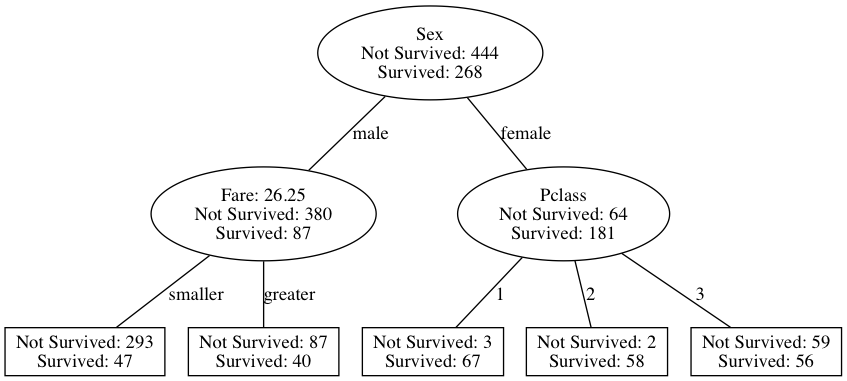
\includegraphics[scale=0.3]{titanic-depth2-c45.png}
    \caption{Titanic decision tree (C4.5)}
    \label{fig:titanic}
\end{figure}

As we can see, some leafs allow for a good classification, e.g.\ for female passengers that traveled in the first two classes (\emph{Pclass} refers to the passenger class). Male passengers have a higher probability of surviving in the first class (ID3) or when they are still very young (C4.5). But other than that, there's too much randomness involved to make good predictions using these two trees.

For missing feature values we tried imputing the mean, as well as using C4.5's built-in solution. The latter sometimes produced models with a minimally better accuracy, but generally the results were in the same ballpark.

To combat overfitting, we implemented the pruning algorithm described in Section~\ref{subsec:c45-pruning}. This improved test accuracy to $0.821$. Pruning removed $147$ of $201$ nodes, so a large part of the tree was actually cut. sklearn managed to get an out of the box accuracy of $0.810$, so this time we managed to comfortably beat sklearn.
Limiting the depth did generally not help a lot, and was vastly outperformed by pruning.

Finally, we tried applying Random Forest to this dataset. The Random Forest variant that uses different data points for each tree performed the worst. After seeing this, we quickly settled to the variant that uses a subset of all features. This generally performed better, but also introduced a large amount of randomness. When training a model with the same parameters several times, the accuracy might be completely different. In the end, we only managed to get the same accuracy as our best C4.5 model (0.8211), by using all features.  We spent some time manually weighting features, but this also did not improve accuracy further.

sklearn got an accuracy of $0.816$ using Random Forest. Our end result is better, but this time, we did a lot of hyperparameter tuning for our own algorithm, and none for sklearn, so it is not a fair comparison to make. Furthermore, sklearn's Random Forest implementation is a lot less vulnerable to randomness, so it is probably a better idea to use this implementation. Since our Random Forest also did not improve on C4.5 itself, we think that our implementation might be too simplistic.

By looking at the visualizations of decision trees, we can manually infer feature importance. Generally, the first feature to split on was always \emph{sex}, which we consider to be the most important feature. The features \emph{Pclass} and \emph{Fare} were both also quite important. However, they are strongly correlated, so having both features available only gives a small advantage. Having \emph{age} available improves accuracy, too. \emph{SibSp} and \emph{Parch} (the number of relatives on board of the ship) were only used very deep inside the tree, and can be considered the least important features.

\subsection{Income Census}

This dataset is from the UCI machine learning repository~\cite{census}. Extraction was done by Barry Becker from the 1994 Census database. The features include personal information, like age, work class, education, and others. The task is to predict whether a person makes over \$50.000 a year.

First, we used the sklearn library to build a decision tree. To avoid overfitting, and to be able to compare the result with ID3, we removed all continuous features. The accuracy is 0.814.

Then we used our own ID3 and C4.5 implementations to construct decision trees with different maximum depths. The accuracy of each tree is shown below in Figure \ref{fig:id3c45all}.
\begin{figure}[h]
	\centering
     \begin{tabular}{c|c|c}
       \textbf{Maximum Depth} & \textbf{ID3} & \textbf{C4.5} \\
       \hline
       2 & 0.822 & 0.829 \\
       3 & 0.823 & 0.837 \\
       4 & 0.818 & 0.835 \\
       5 & 0.817 & 0.831
     \end{tabular}
     \caption{Accuracies for different depths}
     \label{fig:id3c45all}
\end{figure}

Even in the worst case, which is the decision tree constructed by ID3 with maximum depth of five, the accuracy of it is 0.817. It is still higher than the model trained by sklearn, which means that here our module works better than sklearn's module.

We can see that with the growing depth of the decision trees constructed by either ID3 or C4.5, the accuracy first grew, then dropped.

The reason why this situation happened can be that when the maximum depth is smaller than three, both models are underfitting. Once the depth is three, it is the optimal depth for both trees. The accuracies are the highest. And if the maximum depth keeps growing, both models are overfitting. That's why the accuracies start to drop.

The second experiment we did was to use a subset of features for training our decision tree. We assume that the feature \emph{relationship} is redundant to another feature \emph{marital-status} (i.e.\ they are strongly correlated), so we removed only one of them, and tested the model after we trained it. The decision trees in this experiment are all with same maximum depth of 3. The accuracies are shown in Figure \ref{fig:id3c45second}.

\begin{figure}[h]
    \centering
        \begin{tabular}{c|c|c}
        \textbf{Feature excluded} & \textbf{ID3} & \textbf{C4.5} \\
        \hline
        \emph{marital-status} & 0.823 & 0.838 \\
        \emph{relationship} & 0.824 & 0.836 \\
        \emph{marital-status}, \emph{relationship} & 0.787 & 0.798
        \end{tabular}
    \caption{Accuracies when excluding different features}
    \label{fig:id3c45second}
 \end{figure}

Compared to the corresponding accuracies in Figure \ref{fig:id3c45all}, the accuracies with one feature removed in Figure \ref{fig:id3c45second} do not change much. When both features are removed, accuracy drops a lot, so one of the features is needed. This provides more evidence for our assumption that one of the features \emph{relationship} and \emph{marital-status} is redundant.

The third experiment is directly removing the feature \emph{native country}, because this feature includes 41 kind of values in the dataset. With so many detailed values, the model can easily overfit. After we removed it, the accuracy of the decision tree built by ID3 dropped to 0.763, but the accuracy of the decision tree built by C4.5 grows to 0.836. The reason why the accuracy drops in the ID3 tree can probably be that the number of discrete features is only eight, including the feature \emph{native-country}. When we removed the feature \emph{native-country}, there are only seven left. Such few features cause underfitting. This situation does not happen in the C4.5 model, because here there are 12 discrete and continuous features. Even if we remove the feature \emph{native-country}, there are still 11 features left, which means underfitting will not happen. Meanwhile, overfitting is also avoided by the removal of that feature. This is why the accuracy grows to be the highest in the C4.5 model.

The last two experiments are for testing whether Random Forest and pruning improve the accuracy. The final accuracy when using Random Forest is 0.829. The final accuracy when using pruning is 0.846. That is the highest accuracy we achieved, by quite a large margin. The execution time for using pruning is also much longer, it took us around two hours. We conclude that these two methods are only practical for the dataset if one is willing to spend a long time training. The accuracy could maybe even be better, if we would have tried the combination of Random Forest with pruning, and compared its accuracy with others. But because of limited computing resources, we decided to not do this here. For a random forest with ten trees, it would have taken nearly a day to prune all trees.

\begin{figure}[h]
	\centering
    \begin{tabular}{c|c|c|c|c}
    \textbf{sklearn (CART)} & \textbf{ID3} & \textbf{C4.5} & \textbf{C4.5 with pruning} & \textbf{Random Forest} \\
        \hline
        0.814 & 0.823 & 0.837 & 0.846 & 0.829
    \end{tabular}
    \caption{Best accuracies reached}
    \label{fig:withoutnc}
\end{figure}

\section{Conclusion}

During this project phase, we found that decision trees are great when one wants to understand how models actually decide on predictions internally. This turned out to be useful for the analysis part of the project.

ID3 is based on a simple idea, but for our datasets it already performed pretty well. For a short introduction, it also illustrates the foundational ideas nicely.
C4.5 uses much more sophisticated methods. For our datasets, this helped to squeeze out a few percentage points of additional accuracy. Especially dealing with continuous features and pruning are great additions to decision trees. Pruning increases training time a lot, but also performs really well.

To reduce overfitting even more, we explored Random Forest. At least for our analyzed datasets, this did not improve accuracy further. Still, it was interesting to learn about this algorithm. Given more time, it should be possible to implement much more sophisticated variations of it.

Our visualization function turned out to be very useful for debugging our algorithm implementations, as well as figuring out how they deal with the different datasets.

Finally, it is worth noting that there are many aspects of decision trees we did not even touch on. Interested readers might want to explore more about incremental decision tree learning, other uncertainty measures like gini impurity, or other algorithms for building decision trees, like CART~\cite{friedman2001elements}.

\bibliographystyle{ieeetr}
\bibliography{sources}

\end{document}
